\documentclass{beamer}

\usepackage{multicol}
%\usepackage[dvipsnames]{xcolor}
\usepackage{graphicx}
\usepackage{pifont}
\usepackage{multirow}
\usepackage{ragged2e}
\usepackage{changepage}
\usepackage{adjustbox}

\usepackage{wrapfig}

\usepackage[margin=1in, top=1.25in, headheight=2\baselineskip, headsep=\baselineskip]{geometry}


% Grafici
\usepackage{graphicx, booktabs, wrapfig, pdfpages}
\usepackage{pgfplots}
\usepackage[framemethod=tikz]{mdframed}
\usepackage[outline]{contour}
\usepackage[ labelfont=bf, labelsep=period, margin=0.5in]{caption}\usepackage{pdfpages}
\usepackage[labelfont=bf, labelsep=period, margin=0.5in]{caption}

\usepackage{upgreek} %per scrivere mu non corsivo (\upmu)

% Use Unipd as theme, with options:
% - pageofpages: define the separation symbol of the footer page of pages (e.g.: of, di, /, default: of)
% - logo: position another logo near the Unipd logo in the title page (e.g. department logo), passing the second logo path as option 
% Use the environment lastframe to add the endframe text
\usetheme[pageofpages=of]{Unipd}

\title{Proprietà dei candidati Muoni del Trigger L1 di CMS}
%\subtitle{Demonstrating how to use the Unipd theme}
\author[La Rovere Francesco]{La Rovere Francesco}

\date{9 Dicembre, 2024}

\AtBeginSubsection[]
{
  \begin{frame}
  \large

    \frametitle{Indice analitico}
    \tableofcontents[currentsection, subsectionstyle=show/shaded]
  \end{frame}
}

\begin{document}
\footnotesize

% Make the title page
\frame{\titlepage}

\section{Introduzione}

\begin{frame}{LHC e CMS}

Situato a Ginevra, Svizzera, il Large Hadron Collider è il più grande acceleratore di particelle mai costruito. 


\begin{columns}
    \begin{column}{0.55\textwidth}
        \begin{itemize}            
            \item Collisione di particelle a $\sqrt{s} \approx 14$ TeV
            \item Collisioni ogni 25ns $\rightarrow$ rate di interazione 40MHz
        \end{itemize}

        CMS esperimento multifunzionale
        \begin{itemize}
            \item Raccogliere informazioni sulle collisioni di protoni
            \item Selezione eventi $\rightarrow$ sistema di Trigger

        \end{itemize}
    \end{column}
    \begin{column}{0.4\textwidth}  
       \scalebox{0.11}{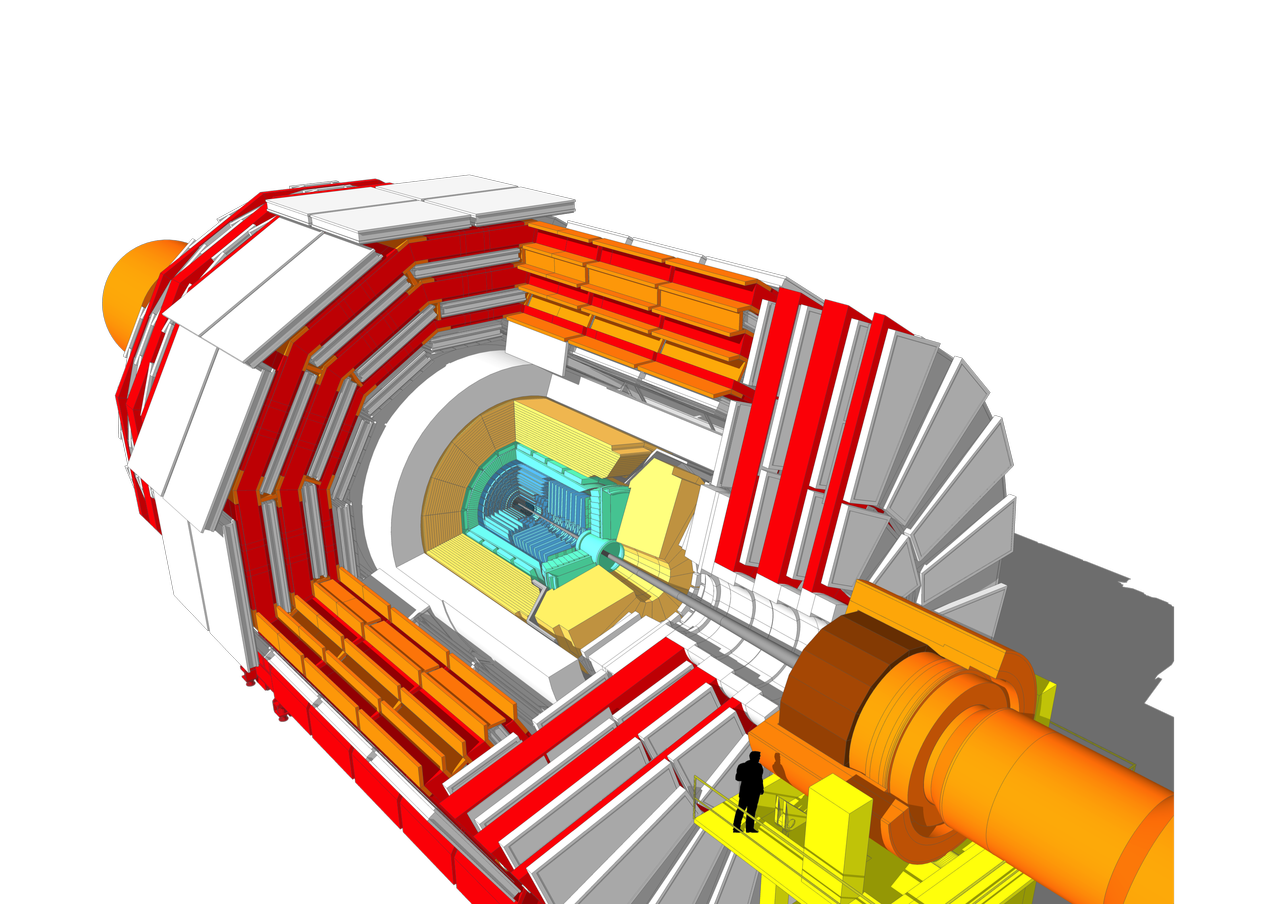
\includegraphics{Immagini/CMS.png}}  
    \end{column}
\end{columns}

\end{frame}



\begin{frame}{Data Scouting}

Il sistema di Trigger scarta la quasi totalità degli eventi, 40MHz $\rightarrow$ 1kHz:


\begin{columns}
    \begin{column}{0.50\textwidth}
        \begin{itemize}            
            \item Introduzione di un bias 
            \item Occultamento di segnali di Nuova Fisica
        \end{itemize}
        \vspace{0.2 cm}
        Sistema di Data Scouting introdotto con la Run 3:
        \begin{itemize}
            \item Analisi della totalità degli eventi nella catena di Trigger
            \item Minore risoluzione, maggiore statistica
            \item Nessun bias

        \end{itemize}
    \end{column}
    \begin{column}{0.4\textwidth}  
    \centering
    \vspace{0.4cm}
       \scalebox{0.16}{\includegraphics{Immagini/TriggerSystemDS.png}}  
    \end{column}
\end{columns}
    
\end{frame}




\section{Proprietà dei candidati Muoni}
\subsection{Validazione delle Trigger  Superprimitives}

\begin{frame}{Trigger Superprimitives}

\begin{columns}

    \begin{column}{0.5\textwidth}
    Nella regione di barrel, $|\eta| < 1.2$:
    \begin{itemize}
        \item Eventi di background minimi
        \item Sono impiegati DT e RPC
    \end{itemize}
    \vspace{0.5 cm}
    Le schede TwinMux:
    \begin{itemize}
        \item Generano superprimitives dai segnali dei DT e RPC
        \item Assegnano a ciascuna superprimitives parametri spaziali e qualitativi.
    \end{itemize}

    \end{column}
    \begin{column}{0.5\textwidth}
        \centering
        \scalebox{0.18}{\includegraphics{Immagini/TriggerSystemTwinMux.png}} 
    \end{column}
\end{columns}
    
\end{frame}



\begin{frame}{Stubs Filling Scheme}

In LHC circolano fasci formati da al massimo 3564 pacchetti discreti di protoni distanti 25ns. La disposizione dei pacchetti è chiamata Filling Scheme.

\vspace{0.8 cm}

\begin{columns}

    \begin{column}{0.5\textwidth}
        \scalebox{0.21}{\includegraphics{Immagini/Stubs/StubsBXnumber.pdf}} 
    \end{column}
    \begin{column}{0.5\textwidth}
        \centering
        \scalebox{0.21}{\includegraphics{Immagini/Stubs/StubsBXnumberZoom.pdf}} 
    \end{column}
\end{columns}

\end{frame}



% \begin{frame}{Stubs Molteplicity}

% Distribuzione della molteplicità di stubs generate dalle schede TwinMux per BX e per orbita.

% \vspace{0.8 cm}

% \begin{columns}

%     \begin{column}{0.5\textwidth}
%         \scalebox{0.21}{\includegraphics{Immagini/Stubs/StubsMolteplicity.pdf}} 
%     \end{column}
%     \begin{column}{0.5\textwidth}
%         \centering
%         \scalebox{0.21}{\includegraphics{Immagini/Stubs/StubsPerOrbit.pdf}} 
%     \end{column}
% \end{columns}

% \end{frame}



\begin{frame}{Stubs Occupancy}

Distribuzione spaziale delle stubs nel corpo di CMS studiando l'occupazione delle Station, Sector e Wheel.

\vspace{0.8 cm}

\begin{columns}

    \begin{column}{0.5\textwidth}
        \scalebox{0.19}{\includegraphics{Immagini/Stubs/StubsSectorWheel.pdf}} 
    \end{column}
    \begin{column}{0.5\textwidth}
        \centering
        \scalebox{0.19}{\includegraphics{Immagini/Stubs/StubsStationWheel.pdf}} 
    \end{column}
\end{columns}

\end{frame}


\subsection{Validazione dei candidati Muoni emulati del BMTF}

\begin{frame}{BMTF Muons}

\begin{columns}

    \begin{column}{0.5\textwidth}
    Ricostruzione del muone avviene in:
    \begin{itemize}
        \item Hardware: sistema di Tracking della regione di barrel BMTF
        \item Software: emulazione del sistema di Tracking
    \end{itemize}
    

    \end{column}
    \begin{column}{0.5\textwidth}
        \centering
        \scalebox{0.18}{\includegraphics{Immagini/TriggerSystemBMTF.png}} 
    \end{column}
\end{columns}

\end{frame}


\begin{frame}{BMTF Molteplicity}

Distribuzione della molteplicità dei candidati muoni emulati in software per BX e per orbita.

\vspace{0.8 cm}

\begin{columns}

    \begin{column}{0.5\textwidth}
        \scalebox{0.21}{\includegraphics{Immagini/BMTF/BMTF_Molteplicity.pdf}} 
    \end{column}
    \begin{column}{0.5\textwidth}
        \centering
        \scalebox{0.21}{\includegraphics{Immagini/BMTF/BMTF_orbit.pdf}} 
    \end{column}
\end{columns}

\end{frame}

\subsection{Confronto Muoni del BMTF con Muoni del GMT}

\begin{frame}{GMT Muons}

\begin{columns}

    \begin{column}{0.5\textwidth}
    Il GMT ha il compito di selezionare i migliori 108 candidati muoni dei 3 sistemi di tracking in base a:
    \begin{itemize}
        \item Qualità
        \item Momento trasverso $p_T$
        \item Provenienza
    \end{itemize}
    \vspace{0.5cm}
    È interessante verificare il confronto tra muoni del GMT, raccolti dal sistema di DS, e candidati muoni emulati del BMTF.
    

    \end{column}
    \begin{column}{0.5\textwidth}
        \centering
        \scalebox{0.18}{\includegraphics{Immagini/TriggerSystemGMT.png}} 
    \end{column}
\end{columns}

\end{frame}


\begin{frame}{Confronto BMTF e GMT Muons}

Il confronto è effettuabile in due modi. In un determinato BX:
\begin{columns}

    \begin{column}{0.5\textwidth}
        \begin{itemize}
            \item Fissare un muone del BMTF e verificare la compatibilità con i muoni del GMT (primo metodo)
            \item Fissare un muone del GMT e verificare la compatibilità con i muoni del BMTF (secondo metodo)
        \end{itemize}
        \vspace{0.5 cm}
        Dove la compatibilità è definita dalla distanza: $\Delta R = \sqrt{(\Delta \phi)^2 + (\Delta \eta)^2} < 0.4$
    \end{column}
    \begin{column}{0.5\textwidth}
        \centering
        \vspace{0.5 cm}
        \scalebox{0.21}{\includegraphics{Immagini/Confronto/DeltaR.pdf}} 
    \end{column}
\end{columns}

\vspace{0.5 cm}
Per il primo metodo la percentuale di eventi con match è 94.42\% mentre per il secondo è 99.72\%

\end{frame}



\begin{frame}{Studio della Matching Efficiency}
\begin{columns}

    \begin{column}{0.55\textwidth}

    Primo metodo:
    \begin{itemize}
        \item Decrescita esponenziale a bassi $p_T$
        \item Crescita logaritmica a $p_T$ maggiori
    \end{itemize}

    Secondo metodo:
    \begin{itemize}
        \item Maggiore matching efficiency a bassi $p_T$
        \item Leggera decrescita a $p_T$ maggiori
    \end{itemize}
        
    \end{column}
    \begin{column}{0.5\textwidth}
        \centering
        \vspace{0.5 cm}
        \scalebox{0.21}{\includegraphics{Immagini/Confronto/PtMatchingEfficiency.pdf}} 
    \end{column}
\end{columns}

\vspace{0.5 cm}

\end{frame}


% \begin{frame}{Studio della Matching Efficiency}

% NON CREDO CHE LA METTERÒ

% \begin{columns}

%     \begin{column}{0.55\textwidth}
%     Studio della qualità dei muoni per entrambi i metodi negli intervalli $p_T \in [0, 5.5]$GeV/c, $p_T \in [100, 255]$GeV/c

%     \vspace{0.3 cm}
%     In entrambi i casi si ha una maggiore qualità per muoni con momento elevato, ovvero un muone con qualità elevata è più probabile avere un momento trasverso elevato.
        
%     \end{column}
%     \begin{column}{0.45\textwidth}
%         \centering
%         \scalebox{0.16}{\includegraphics{Immagini/Confronto/QualLowHighPt.pdf}} 
%         \vspace{0.5 cm}
%         \scalebox{0.16}{\includegraphics{Immagini/Confronto/GMTQualLowHighPt.pdf}} 
%     \end{column}
% \end{columns}

% \vspace{0.5 cm}

% \end{frame}




\section{Nuova Fisica a CMS}
\subsection{Ricerca Heavy Stable Charged Particles}

\begin{frame}{HSCPs a CMS}
    Tecnica di Data Scouting $\rightarrow$ acquisizione dati unbiased a 40MHz:
    \begin{itemize}
        \item Ricerca di particelle non predette dal Modello Standard
    \end{itemize}

    \vspace{0.3 cm}
    
    Heavy Stable Charged Particles sono particelle Long Lived con masse di svariate centinaia di GeV/$c^2$. Principali firme sperimentali:
    \begin{itemize}
        \item Velocità ridotta $\beta \ll 1$
        \item \textbf{Elevato tempo di volo}
        \item Anormale perdita di energia per unità di lunghezza $\langle \frac{dE}{dx}\rangle$
    \end{itemize}

    \vspace{0.3 cm}

    Si cercano segnali di particelle (stubs) che impiegano più di 1BX per attraversare CMS, ovvero:
    \begin{itemize}
        \item Stubs nel BX+1 nella stazione sucessiva rispetto alla stubs nel BX
        \item Stubs bel BX+1 nello stesso sector e wheel, o in quelli adiacenti, rispetto alla stubs nel BX
    \end{itemize}
\end{frame}



\subsection{Studio delle Stubs}
\begin{frame}{Matched Stubs}

Distribuzione delle stubs totali compatibili tra BX e BX+1. Il rate di stubs con match corrisponde a 2.2kHz. 

\vspace{0.6cm}

\begin{columns}

    \begin{column}{0.5\textwidth}
        \scalebox{0.21}{\includegraphics{Immagini/HSCP/MatchedStubs.pdf}} 
    \end{column}
    \begin{column}{0.5\textwidth}
        \scalebox{0.215}{\includegraphics{Immagini/HSCP/MatchedStubsCombination.pdf}} 
    \end{column}
\end{columns}

\vspace{0.5 cm}
    
\end{frame}


\subsection{Studio dei candidati Muoni}

\begin{frame}{Matched BMTF muons}

Studio delle coppie candidati muoni del BMTF in BX adiacenti generati da quattro stubs compatibili (due ognuno):

\begin{columns}

    \begin{column}{0.55\textwidth}
    \begin{itemize}
        \item Rappresentanti probabilmente lo stesso evento
        \item Percepiti dal Trigger come due particelle distinte
    \end{itemize}

    Eventi molto rari, rate $\approx$ 1.4Hz.

    \begin{itemize}
        \item Verificare se sono eventi generati dalla collisione di protoni
        \item Verificare le distribuzioni spaziali e di momento delle coppie di muoni
    \end{itemize}
        
    \end{column}
    \begin{column}{0.5\textwidth}
        \scalebox{0.205}{\includegraphics{Immagini/HSCP/BXDiff.pdf}} 
    \end{column}
\end{columns}
    
\end{frame}


\begin{frame}{Matched BMTF muons}

Distribuzione dei momenti relativi $\frac{p_T^{BX} - p_T^{BX+1}}{p_T^{BX}}$ e spaziale $\phi^{BX} - \phi^{BX+1}$ delle coppie di muoni del BMTF in BX adiacenti

\vspace{0.8cm}

\begin{columns}

    \begin{column}{0.5\textwidth}
        \scalebox{0.21}{\includegraphics{Immagini/HSCP/DeltaPt.pdf}}  
    \end{column}
    \begin{column}{0.5\textwidth}
        \scalebox{0.21}{\includegraphics{Immagini/HSCP/DeltaPhi.pdf}} 
        
    \end{column}
\end{columns}
    
\end{frame}



    
    
\end{document}